\section{Phân tích tổng quan}
\subsection{Các khái niệm liên quan trong đề tài}

\subsubsection{Co-working Space}

Co-working Space (không gian làm việc chung) là mô hình cung cấp môi trường làm việc linh hoạt cho cá nhân, freelancer, nhóm khởi nghiệp, doanh nghiệp nhỏ và các chuyên gia độc lập. Thay vì phải thuê một văn phòng riêng với chi phí cố định lớn, khách hàng có thể lựa chọn sử dụng chỗ ngồi, phòng họp, văn phòng riêng hoặc các khu vực làm việc chung theo nhu cầu thực tế.

Không gian làm việc chung thường được trang bị các tiện ích phục vụ công việc như Wi-Fi tốc độ cao, bàn ghế làm việc, phòng họp, máy in, máy chiếu, khu vực tiếp khách và các dịch vụ hỗ trợ văn phòng. Bên cạnh việc cung cấp địa điểm làm việc, mô hình này còn tạo ra môi trường kết nối cộng đồng, giúp các thành viên có cơ hội giao lưu, chia sẻ kinh nghiệm, tìm kiếm đối tác và hợp tác trong công việc.

Trong phạm vi đề tài, Co-working Space là đối tượng chính được hệ thống hỗ trợ quản lý. Hệ thống cần cho phép ban quản lý theo dõi thông tin không gian, chỗ ngồi, phòng họp, gói dịch vụ, khách hàng, hợp đồng thuê, lịch sử đặt chỗ và tình trạng sử dụng dịch vụ. Đồng thời, khách hàng có thể sử dụng hệ thống để đặt chỗ, đăng ký gói dịch vụ, quản lý lịch sử sử dụng và tham gia các hoạt động kết nối trong cộng đồng làm việc chung.

\subsubsection{Đặc điểm của mô hình Co-working Space}

Co-working Space không chỉ là nơi cung cấp chỗ ngồi làm việc mà còn là một mô hình dịch vụ văn phòng linh hoạt. Khách hàng có thể lựa chọn sử dụng không gian theo giờ, ngày, tuần hoặc tháng tùy theo nhu cầu, thay vì phải ký hợp đồng thuê văn phòng dài hạn. Điều này giúp giảm chi phí vận hành, đặc biệt phù hợp với freelancer, nhóm khởi nghiệp, doanh nghiệp nhỏ và các cá nhân thường xuyên làm việc theo dự án.

Một Co-working Space thường bao gồm nhiều loại tài nguyên khác nhau như khu vực làm việc chung, chỗ ngồi cố định, phòng họp, văn phòng riêng, khu vực tiếp khách và các tiện ích hỗ trợ công việc. Các tài nguyên này cần được quản lý về số lượng, trạng thái sử dụng, lịch đặt chỗ, thời gian thuê và chi phí sử dụng. Vì vậy, việc ứng dụng hệ thống thông tin vào quản lý Co-working Space giúp ban quản lý kiểm soát hiệu quả hoạt động khai thác không gian, hạn chế trùng lịch đặt chỗ và nâng cao chất lượng phục vụ khách hàng.

Ngoài yếu tố không gian, Co-working Space còn chú trọng đến việc xây dựng cộng đồng người dùng. Các thành viên trong cùng một không gian làm việc có thể đến từ nhiều lĩnh vực khác nhau, có kỹ năng, kinh nghiệm và nhu cầu hợp tác khác nhau. Do đó, hệ thống không chỉ hỗ trợ các nghiệp vụ quản lý đặt chỗ, gói dịch vụ, hợp đồng và thanh toán, mà còn cần hỗ trợ người dùng khai báo hồ sơ cá nhân, lĩnh vực chuyên môn, kỹ năng, nhu cầu hợp tác và từ khóa quan tâm để tìm kiếm hoặc gợi ý đối tác phù hợp.

\subsubsection{Sự khác biệt giữa Co-working Space và văn phòng truyền thống}

Co-working Space và văn phòng truyền thống đều phục vụ nhu cầu làm việc, họp nhóm và vận hành hoạt động kinh doanh. Tuy nhiên, hai mô hình này có sự khác biệt rõ rệt về cách thức sử dụng không gian, chi phí, mức độ linh hoạt và khả năng kết nối cộng đồng.

\begin{itemize}
    \item \textbf{Mức độ linh hoạt:} Co-working Space cho phép khách hàng sử dụng chỗ ngồi, phòng họp hoặc văn phòng riêng theo giờ, ngày, tuần hoặc tháng. Văn phòng truyền thống thường yêu cầu thuê cố định trong thời gian dài và khó thay đổi quy mô trong ngắn hạn.
    \item \textbf{Chi phí sử dụng:} Co-working Space giúp khách hàng giảm chi phí đầu tư ban đầu vì các tiện ích văn phòng cơ bản đã được cung cấp sẵn. Văn phòng truyền thống thường phát sinh thêm chi phí thuê mặt bằng, trang thiết bị, bảo trì, điện, nước, Internet và nhân sự vận hành.
    \item \textbf{Đối tượng sử dụng:} Co-working Space phù hợp với freelancer, startup, nhóm dự án, doanh nghiệp nhỏ và cá nhân cần nơi làm việc linh hoạt. Văn phòng truyền thống thường phù hợp với doanh nghiệp có quy mô ổn định, cơ cấu tổ chức rõ ràng và nhu cầu sử dụng không gian lâu dài.
    \item \textbf{Quản lý tài nguyên:} Co-working Space có nhiều loại tài nguyên dùng chung như chỗ ngồi, phòng họp, thiết bị và gói dịch vụ nên cần quản lý trạng thái sử dụng, lịch đặt và thanh toán theo từng lượt hoặc từng gói. Văn phòng truyền thống thường ít phát sinh nghiệp vụ đặt chỗ hằng ngày vì không gian đã được phân bổ cố định cho từng bộ phận.
    \item \textbf{Kết nối cộng đồng:} Co-working Space tạo điều kiện để các thành viên gặp gỡ, trao đổi kinh nghiệm và tìm kiếm cơ hội hợp tác. Văn phòng truyền thống chủ yếu phục vụ nội bộ một tổ chức nên khả năng kết nối giữa nhiều nhóm độc lập thường hạn chế hơn.
\end{itemize}

Từ những đặc điểm trên, có thể thấy hệ thống quản lý Co-working Space cần tập trung vào các nghiệp vụ cốt lõi như quản lý không gian làm việc, phòng họp, chỗ ngồi, gói dịch vụ, khách hàng, hợp đồng thuê, lịch sử đặt chỗ, thanh toán, báo cáo doanh thu và mức độ sử dụng dịch vụ. Bên cạnh đó, hệ thống còn cần hỗ trợ xây dựng cộng đồng thành viên thông qua chức năng khai báo hồ sơ cá nhân, kỹ năng, lĩnh vực chuyên môn, nhu cầu hợp tác và gợi ý đối tác phù hợp.

\subsection{Các hệ thống tương tự}

\subsubsection{Hệ thống Regus}

\subsubsubsection{Giới thiệu}

Regus là một trong những mạng lưới cung cấp không gian làm việc chung (co-working space) và văn phòng dịch vụ có quy mô lớn trên thế giới, thuộc sở hữu của tập đoàn toàn cầu IWG plc. Tại thị trường Việt Nam, Regus vận hành nhiều chi nhánh tại các tòa nhà văn phòng ở những khu vực trung tâm như Hà Nội và Thành phố Hồ Chí Minh.

Đối tượng khách hàng mục tiêu của Regus chủ yếu là doanh nghiệp đa quốc gia, tập đoàn lớn, doanh nghiệp vừa và nhỏ hoặc các chuyên gia có nhu cầu sử dụng môi trường làm việc chuyên nghiệp, bảo mật và đồng bộ theo tiêu chuẩn quốc tế. Không gian tại Regus được thiết kế theo hướng văn phòng dịch vụ hiện đại, chú trọng sự yên tĩnh, riêng tư và ổn định nhằm hỗ trợ hoạt động làm việc của cá nhân lẫn tổ chức. Người dùng có thể tra cứu thông tin địa điểm, loại hình không gian và dịch vụ thông qua cổng thông tin trực tuyến tại địa chỉ regus.com.

\begin{figure}[H]
    \centering
    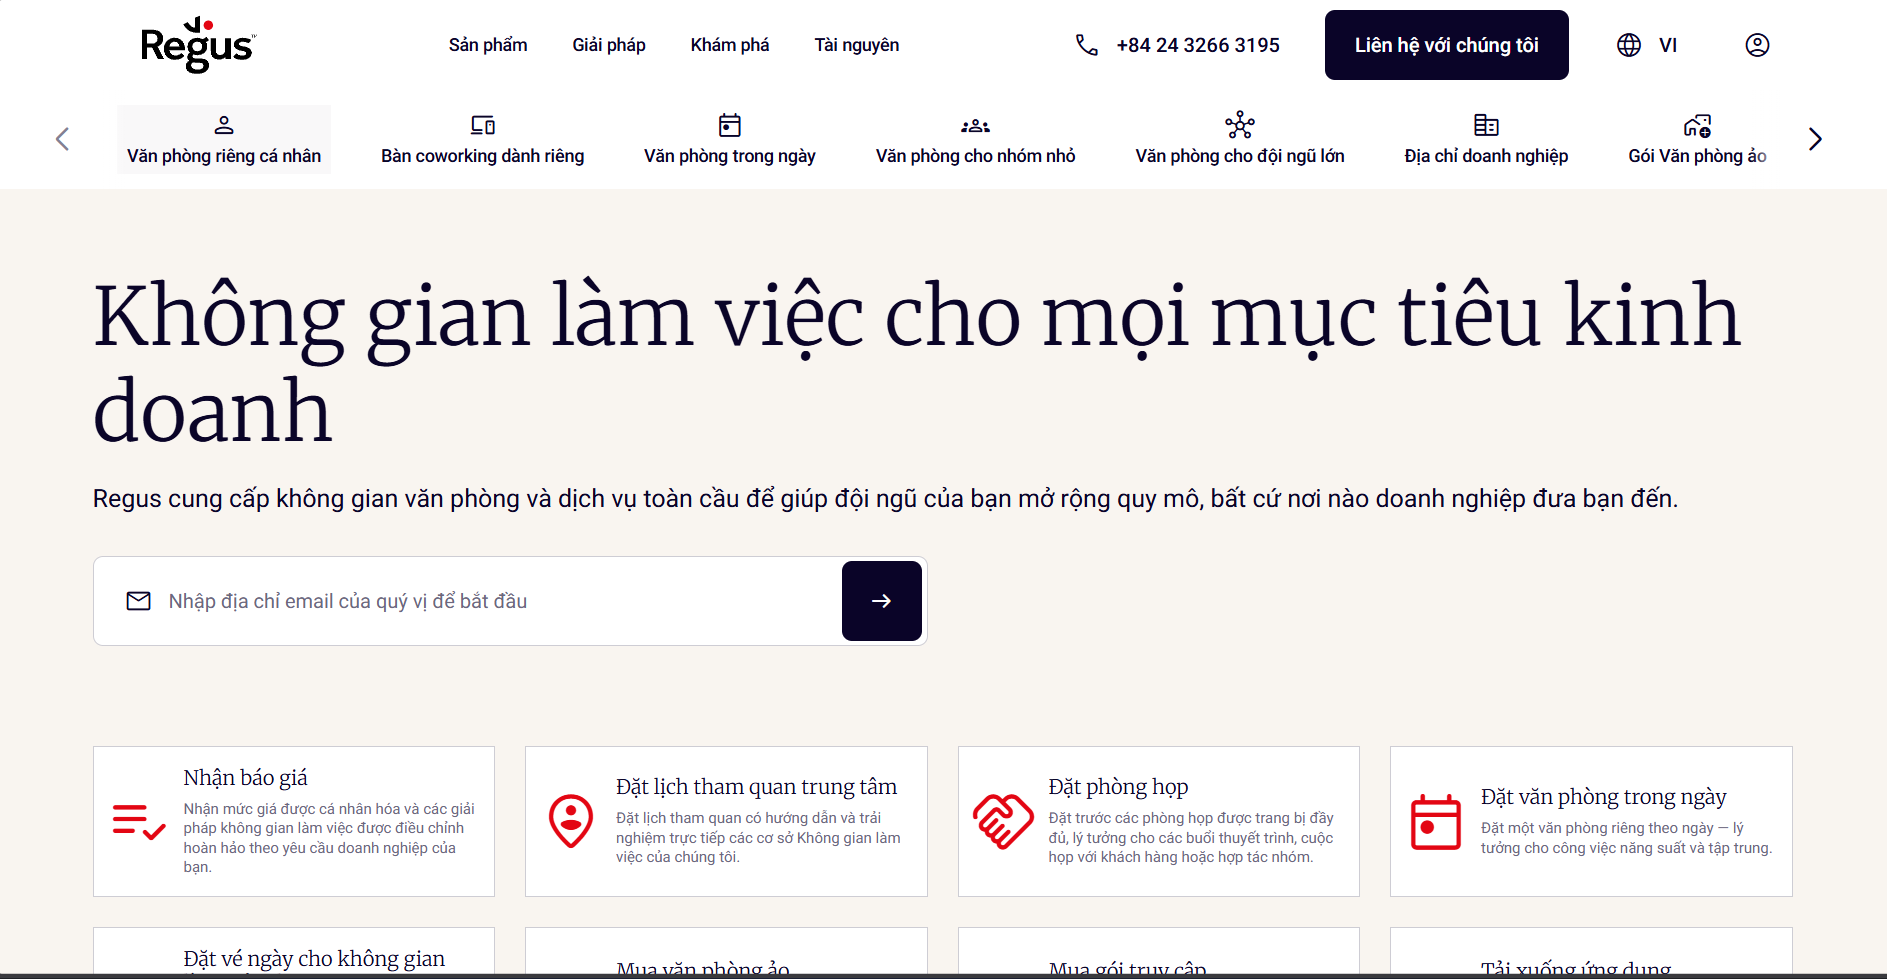
\includegraphics[width=0.85\textwidth]{Images/Chuong2/regus-homepage.png}
    \caption{Giao diện trang chủ cổng thông tin trực tuyến của Regus}
    \label{fig:regus-intro}
\end{figure}

\subsubsubsection{Phân tích}

Nền tảng trực tuyến của Regus, bao gồm website và ứng dụng di động, được xây dựng theo hướng chuẩn hóa trên phạm vi nhiều quốc gia. Hệ thống tập trung hỗ trợ người dùng tìm kiếm địa điểm làm việc, lựa chọn loại hình dịch vụ và thực hiện các thao tác liên quan đến đặt chỗ hoặc liên hệ tư vấn. Một số chức năng nổi bật có thể kể đến như:

\begin{itemize}
    \item Hỗ trợ tìm kiếm không gian làm việc theo khu vực, thành phố hoặc quốc gia, phù hợp với nhu cầu sử dụng đa chi nhánh của khách hàng doanh nghiệp.
    \item Cung cấp thông tin về nhiều loại hình dịch vụ như văn phòng riêng, chỗ ngồi làm việc chung, phòng họp, văn phòng ảo và gói thành viên.
    \item Cho phép người dùng tra cứu thông tin chi tiết về địa điểm, tiện ích, hình ảnh không gian và phương thức liên hệ để đặt dịch vụ.
    \item Hỗ trợ tài khoản khách hàng để theo dõi dịch vụ đã sử dụng, lịch đặt chỗ và các thông tin liên quan đến giao dịch.
\end{itemize}

Về mặt giao diện, hệ thống mang phong cách doanh nghiệp với bố cục rõ ràng, màu sắc trung tính và thanh điều hướng được tổ chức theo từng nhóm dịch vụ. Trải nghiệm người dùng được thiết kế nhất quán, phù hợp với các tổ chức cần tìm kiếm và điều phối không gian làm việc ở nhiều địa điểm khác nhau.

\begin{figure}[H]
    \centering
    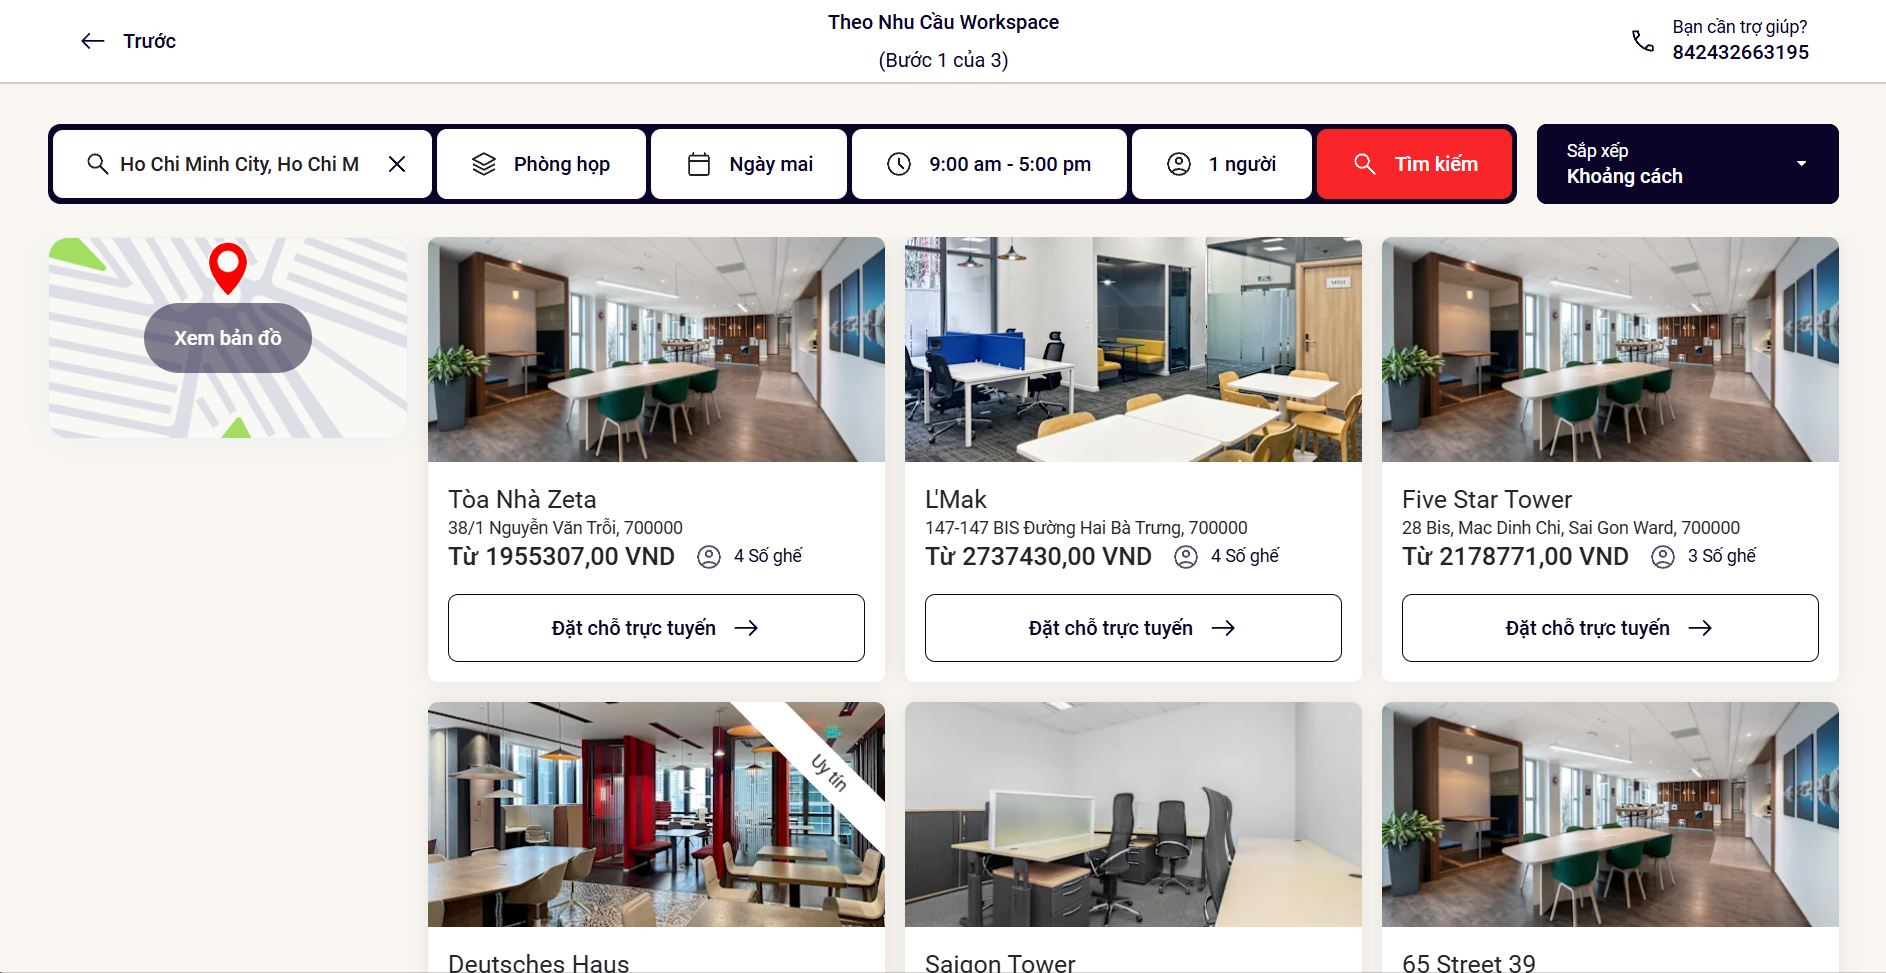
\includegraphics[width=0.85\textwidth]{Images/Chuong2/regus-booking.png}
    \caption{Giao diện luồng đặt phòng họp trực tuyến của Regus}
    \label{fig:regus-analysis}
\end{figure}

\subsubsubsection{Hạn chế}

Mặc dù có hệ thống vận hành quy mô lớn và tính chuẩn hóa cao, nền tảng trực tuyến của Regus vẫn tồn tại một số hạn chế khi áp dụng cho nhóm khách hàng cá nhân, freelancer hoặc startup vừa và nhỏ tại thị trường Việt Nam:

\begin{itemize}
    \item \textbf{Thiếu trực quan trong mô hình hóa không gian:} Luồng đặt chỗ chủ yếu trình bày thông tin dưới dạng danh sách và hình ảnh mô tả. Hệ thống chưa thể hiện rõ sơ đồ mặt bằng tương tác theo thời gian thực, khiến người dùng khó hình dung chính xác vị trí chỗ ngồi, hướng phòng hoặc khoảng cách đến các khu vực tiện ích trước khi đặt chỗ.
    \item \textbf{Chưa tối ưu cho nhu cầu thuê ngắn hạn linh hoạt:} Regus phù hợp với khách hàng doanh nghiệp và các gói dịch vụ chuyên nghiệp, nhưng quy trình tiếp cận dịch vụ có thể chưa thật sự thuận tiện đối với người dùng vãng lai chỉ có nhu cầu thuê theo giờ hoặc theo ngày.
    \item \textbf{Thiếu bản địa hóa trong phương thức thanh toán:} Một số quy trình thanh toán và xác nhận dịch vụ vẫn thiên về mô hình khách hàng doanh nghiệp hoặc thẻ thanh toán quốc tế, chưa nhấn mạnh các phương thức phổ biến tại Việt Nam như ví điện tử, chuyển khoản nhanh hoặc quét mã QR.
    \item \textbf{Thiếu phân hệ tương tác và kết nối cộng đồng số:} Hệ thống tập trung nhiều vào quản lý tài sản không gian và cung cấp dịch vụ thuê văn phòng. Người dùng chưa có công cụ nổi bật để khai báo hồ sơ năng lực, tìm kiếm cộng sự hoặc nhận gợi ý kết nối đối tác dựa trên kỹ năng chuyên môn.
\end{itemize}

\subsubsection{Hệ thống WorkFlow Space}

\subsubsubsection{Giới thiệu}

WorkFlow Space là một mô hình không gian làm việc hướng đến sự linh hoạt, tiện nghi và trải nghiệm người dùng hiện đại. Hệ thống phục vụ các nhóm khách hàng như freelancer, người làm việc từ xa, học sinh, sinh viên, nhóm dự án nhỏ và các cá nhân cần một môi trường làm việc ổn định tại Thành phố Hồ Chí Minh.

Điểm đặc trưng của WorkFlow Space là phong cách thiết kế hiện đại, tối giản, kết hợp không gian mở với các khu vực làm việc yên tĩnh. Không gian được trang bị các tiện ích cần thiết như Internet tốc độ cao, bàn ghế phù hợp cho làm việc trong thời gian dài, khu vực họp nhóm và các dịch vụ hỗ trợ làm việc. Người dùng có thể tìm hiểu thông tin về không gian, bảng giá và dịch vụ thông qua cổng thông tin trực tuyến tại địa chỉ workflowspace.vn.

\begin{figure}[H]
    \centering
    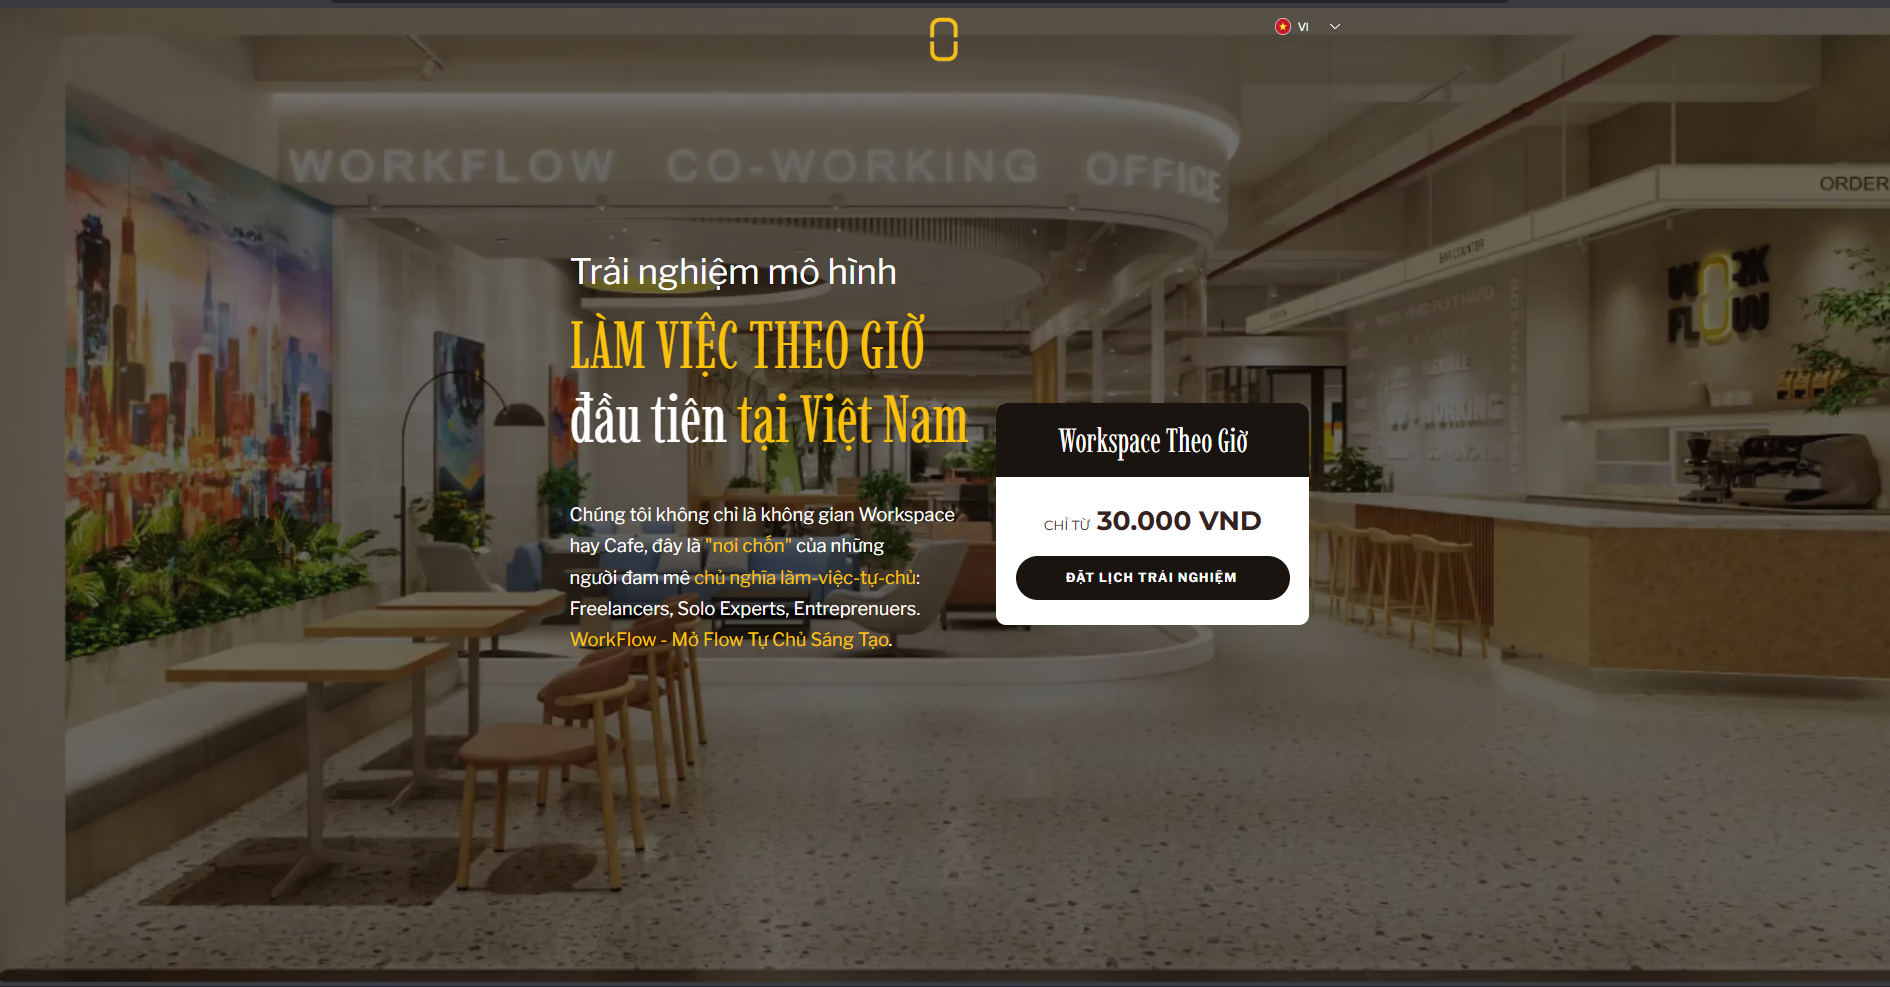
\includegraphics[width=0.85\textwidth]{Images/Chuong2/workflow-intro.png}
    \caption{Không gian làm việc tại WorkFlow Space}
    \label{fig:workflow-intro}
\end{figure}

\subsubsubsection{Phân tích}

Nền tảng trực tuyến của WorkFlow Space được xây dựng theo hướng giới thiệu trực quan về không gian và dịch vụ. Website tập trung vào việc cung cấp thông tin cho người dùng cuối, giúp khách hàng dễ dàng nắm bắt đặc điểm không gian, loại hình dịch vụ và chi phí sử dụng trước khi liên hệ hoặc đăng ký. Các chức năng chính bao gồm:

\begin{itemize}
    \item Hiển thị thông tin về hình ảnh, vị trí, thời gian hoạt động và đặc điểm không gian làm việc.
    \item Cung cấp mô tả và bảng giá của các gói dịch vụ linh hoạt như gói theo giờ, gói theo ngày, thuê phòng họp hoặc thuê không gian dài hạn.
    \item Giới thiệu các tiện ích hỗ trợ làm việc như khu vực họp, không gian yên tĩnh, Internet tốc độ cao và các dịch vụ đi kèm.
    \item Cho phép người dùng đăng ký nhận tư vấn hoặc liên hệ trực tuyến đối với nhu cầu thuê dài hạn, thuê phòng họp hoặc tổ chức sự kiện.
\end{itemize}

Về mặt giao diện, website sử dụng hình ảnh chất lượng cao, bố cục rõ ràng và phong cách trình bày hiện đại. Nội dung được tổ chức theo các nhóm thông tin như không gian, dịch vụ, bảng giá và liên hệ, giúp người dùng dễ dàng tra cứu các thông tin cần thiết trước khi quyết định sử dụng dịch vụ.

\begin{figure}[H]
    \centering
    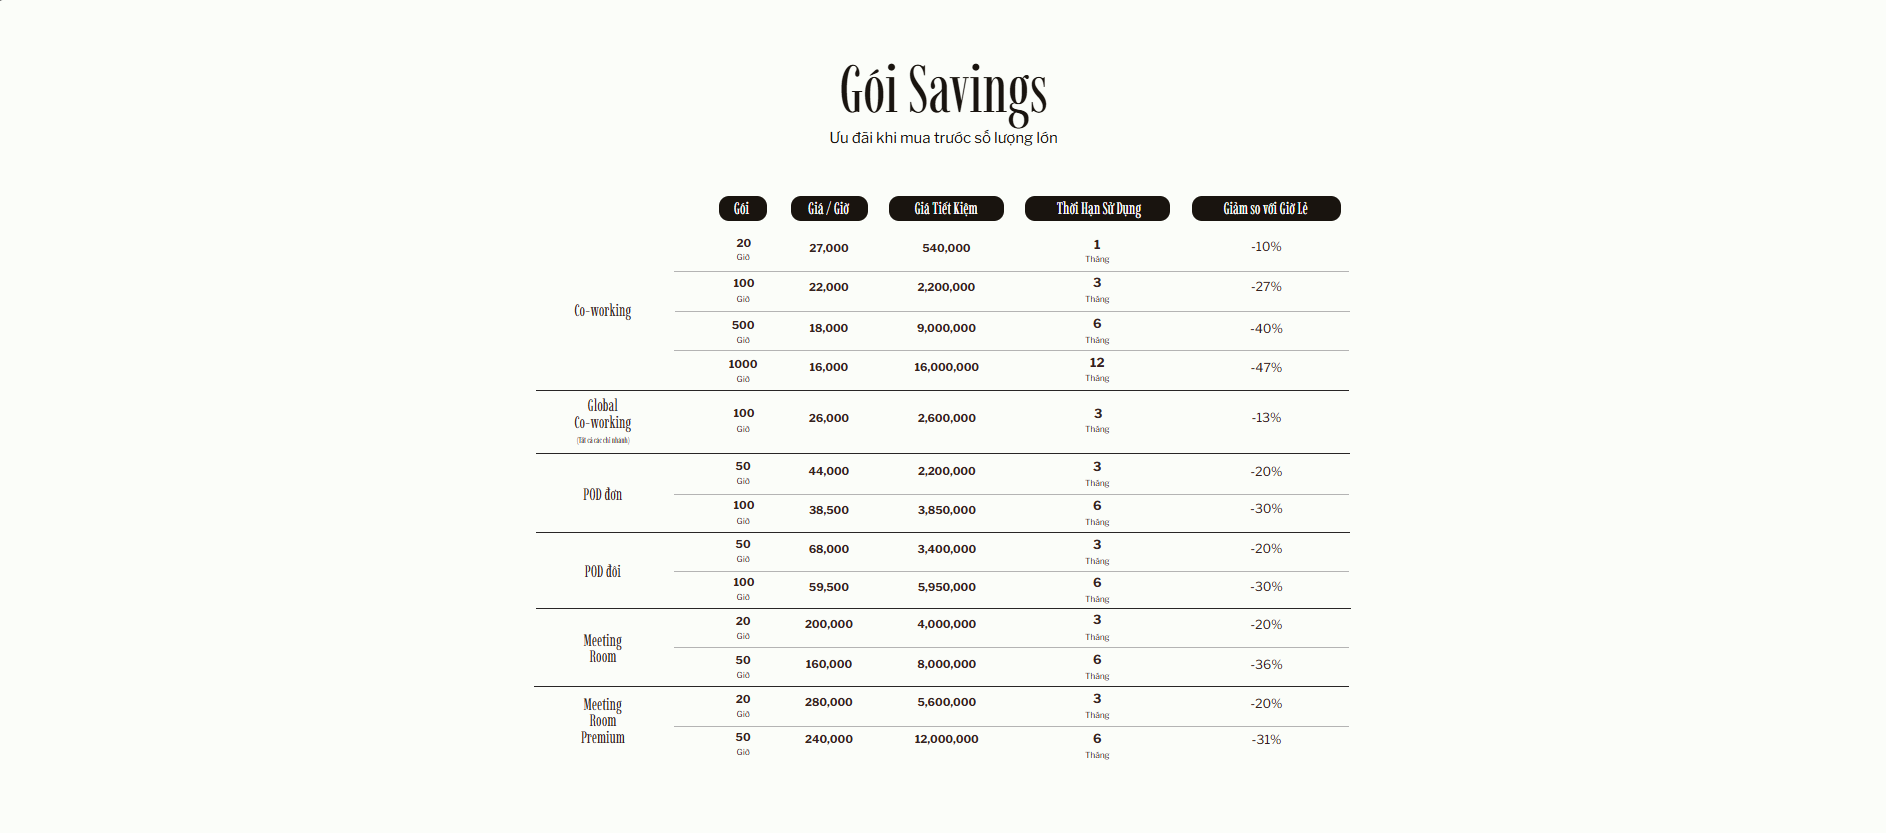
\includegraphics[width=0.85\textwidth]{Images/Chuong2/workflow-pricing.png}
    \caption{Bảng giá các gói dịch vụ trên website WorkFlow Space}
    \label{fig:workflow-analysis}
\end{figure}

\subsubsubsection{Hạn chế}

Dù có giao diện trực quan và cung cấp thông tin dịch vụ tương đối đầy đủ, hệ thống trực tuyến của WorkFlow Space vẫn còn một số hạn chế về khả năng tương tác và tự động hóa quy trình:

\begin{itemize}
    \item \textbf{Hạn chế trong đặt chỗ thời gian thực:} Website chủ yếu đóng vai trò giới thiệu không gian và dịch vụ. Người dùng chưa thể trực tiếp xem trạng thái từng chỗ ngồi hoặc phòng họp theo thời gian thực để đặt chỗ và thanh toán ngay trên hệ thống.
    \item \textbf{Quy trình quản lý hợp đồng chưa được số hóa hoàn toàn:} Đối với các gói thuê dài hạn, quy trình vẫn phụ thuộc nhiều vào biểu mẫu liên hệ và tư vấn thủ công, chưa hỗ trợ đầy đủ việc tạo lập, theo dõi thời hạn và gia hạn hợp đồng trực tuyến.
    \item \textbf{Thiếu tính năng tích hợp đa dịch vụ trong cùng một luồng giao dịch:} Các dịch vụ bổ sung như sử dụng thiết bị, in ấn hoặc tiện ích văn phòng chưa được tích hợp rõ ràng vào quá trình đặt chỗ, khiến trải nghiệm sử dụng dịch vụ chưa thật sự liền mạch.
    \item \textbf{Chưa hỗ trợ nền tảng kết nối cộng đồng số:} Hệ thống mới tập trung vào việc giới thiệu dịch vụ và tiếp nhận thông tin liên hệ. Người dùng chưa có không gian để tạo hồ sơ cá nhân, khai báo kỹ năng, tìm kiếm cộng sự hoặc nhận gợi ý kết nối đối tác dựa trên lĩnh vực chuyên môn.
\end{itemize}



\subsubsection{Hệ thống CirCO}

\subsubsubsection{Giới thiệu}

CirCO là một trong những thương hiệu co-working space nội địa tiên phong và có uy tín lớn tại thị trường Việt Nam, đặc biệt là tại khu vực Thành phố Hồ Chí Minh. Được thành lập với sứ mệnh hỗ trợ hệ sinh thái khởi nghiệp, đối tượng khách hàng mục tiêu của CirCO tập trung mạnh vào các công ty công nghệ, các startup, doanh nghiệp vừa và nhỏ (SMEs) cùng cộng đồng những người làm việc tự do (freelancer).

Không gian của CirCO mang phong cách thiết kế năng động, tối ưu hóa các khu vực sinh hoạt chung nhằm kích thích sự sáng tạo và giao lưu giữa các thành viên. Ngoài hạ tầng cơ bản về chỗ ngồi linh hoạt, phòng họp và văn phòng riêng, CirCO còn nổi tiếng với việc xây dựng một hệ sinh thái hỗ trợ doanh nghiệp thông qua các sự kiện kết nối. Người dùng có thể tìm hiểu thông tin, trải nghiệm luồng dịch vụ trực tuyến của đơn vị thông qua hệ thống cổng thông tin tại địa chỉ circo.co.

\begin{figure}[H]
    \centering
    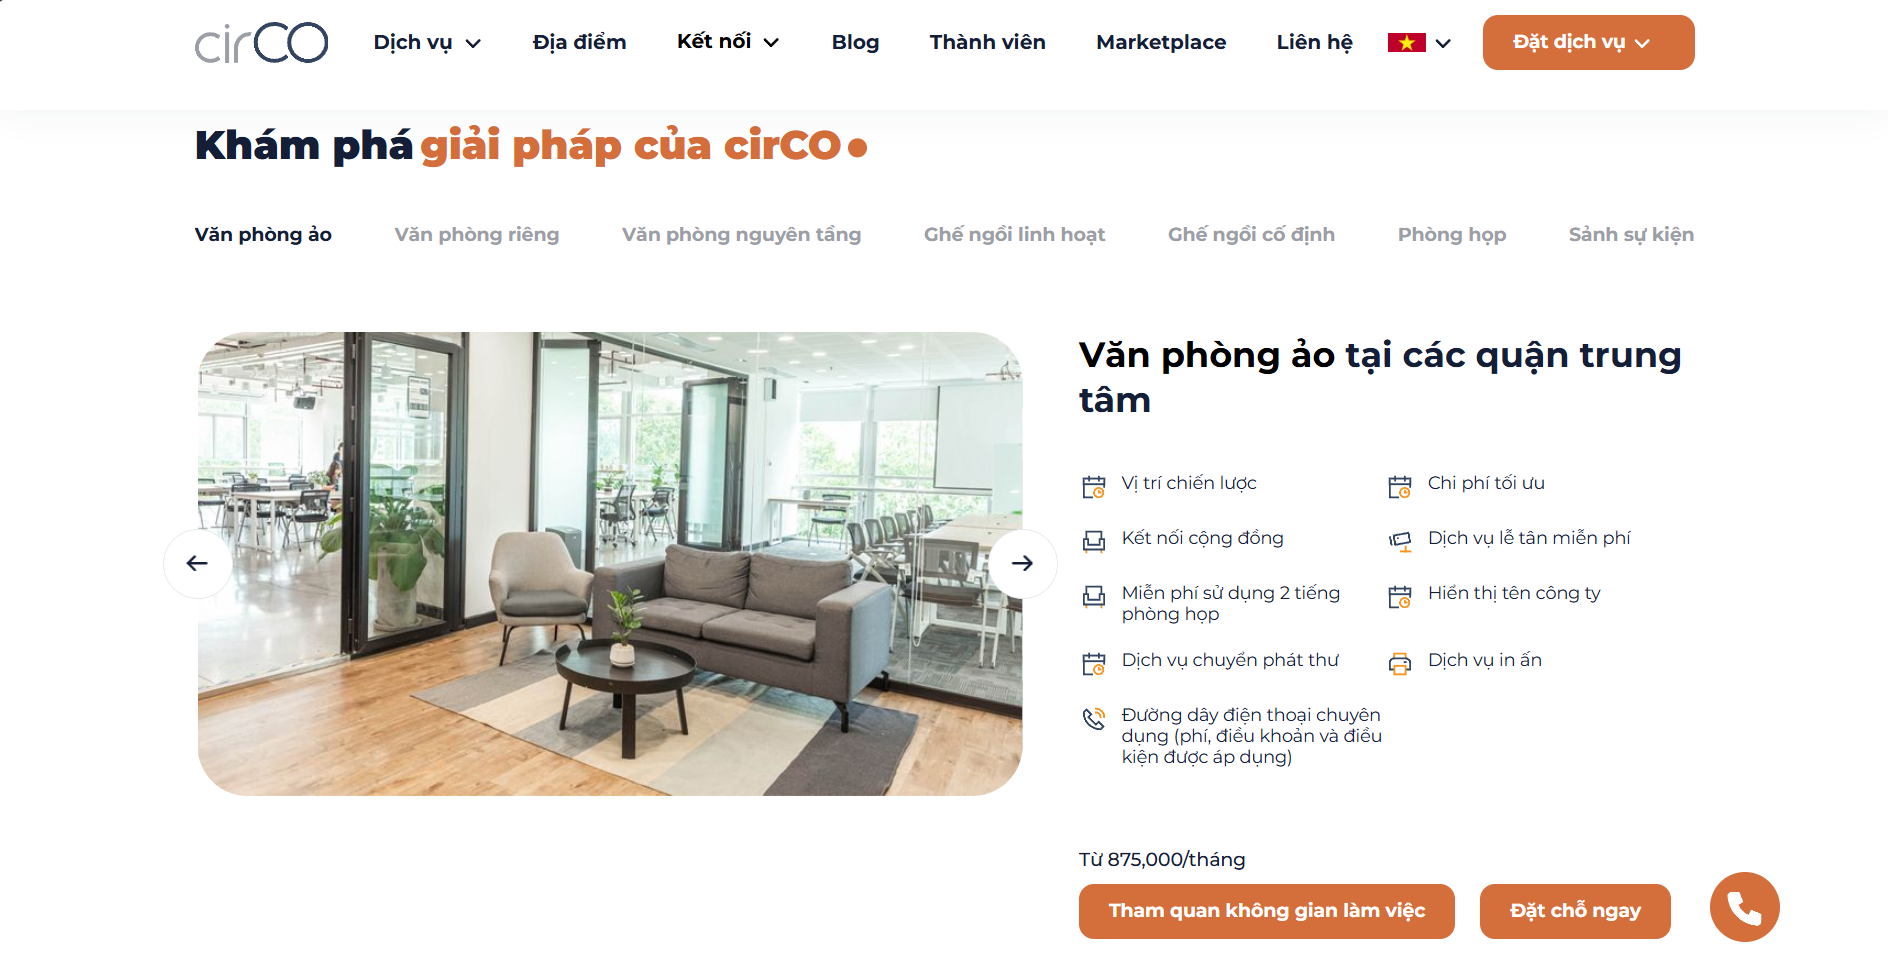
\includegraphics[width=0.85\textwidth]{Images/Chuong2/circo-homepage.png}
    \caption{Giao diện giới thiệu không gian và chi nhánh trên website CirCO}
    \label{fig:circo-intro}
\end{figure}

\subsubsubsection{Phân tích}

Hệ thống trực tuyến của CirCO đã được đầu tư bài bản về mặt tính năng, chuyển đổi từ một trang web giới thiệu thông tin thuần túy sang một nền tảng hỗ trợ giao dịch trực tuyến với các đặc điểm nổi bật:

\begin{itemize}
    \item \textbf{Tích hợp luồng đặt chỗ trực tuyến (Instant Booking):} Người dùng có thể chủ động lựa chọn chi nhánh, loại dịch vụ như phòng họp hoặc chỗ ngồi theo ngày, chọn khung giờ và tiến hành đặt chỗ trực tiếp trên hệ thống mà không cần qua các bước tư vấn gián tiếp.
    \item \textbf{Đa dạng hóa hình thức thanh toán bản địa:} Hệ thống tích hợp tương đối tốt các cổng thanh toán phổ biến tại Việt Nam, cho phép khách hàng thanh toán nhanh qua thẻ nội địa, thẻ quốc tế hoặc quét mã ví điện tử.
    \item \textbf{Quản lý thông tin minh bạch:} Cung cấp giao diện trực quan về bảng giá, mô tả trang thiết bị đi kèm của từng phòng họp, giúp khách hàng dễ dàng so sánh và đưa ra lựa chọn phù hợp với nhu cầu.
\end{itemize}

Về mặt UI/UX, website sở hữu phong cách thiết kế hiện đại, trẻ trung với độ tương phản màu sắc cao, làm nổi bật được không gian làm việc thực tế thông qua các hình ảnh sắc nét. Tốc độ phản hồi của luồng đặt chỗ tương đối nhanh, mang lại trải nghiệm thương mại điện tử mượt mà cho người dùng cuối.

\begin{figure}[H]
    \centering
    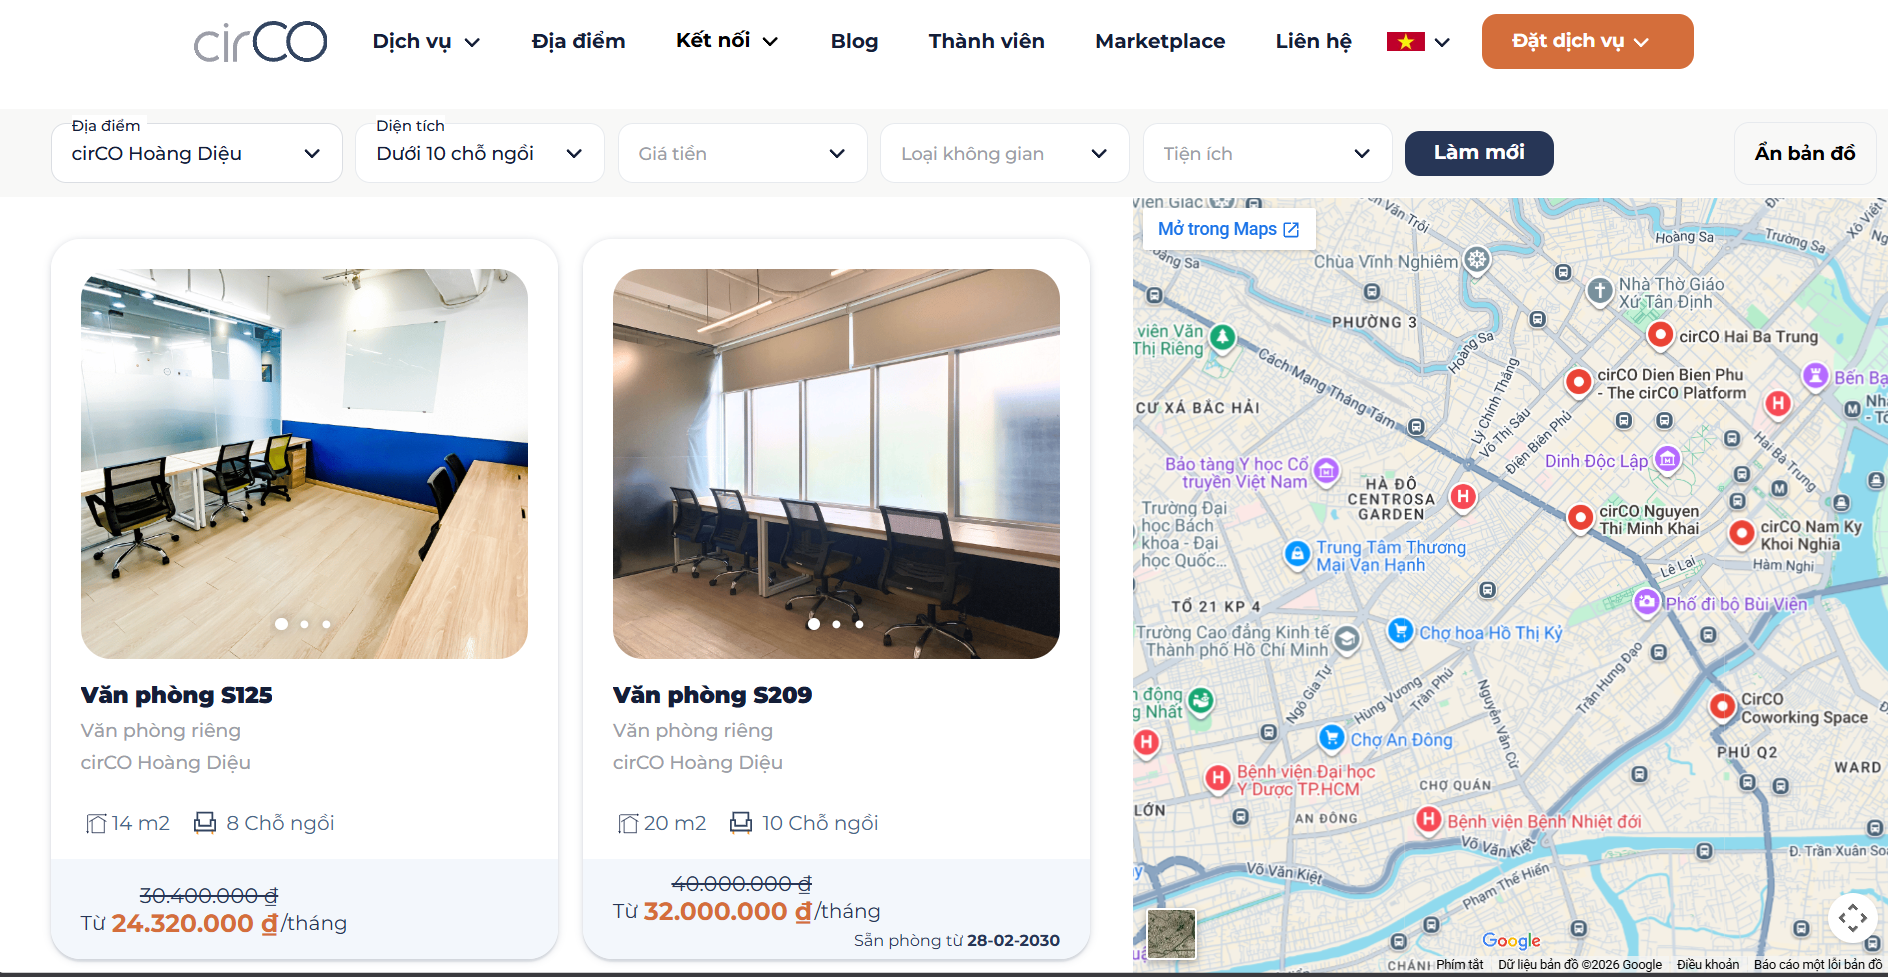
\includegraphics[width=0.85\textwidth]{Images/Chuong2/circo-booking-system.png}
    \caption{Giao diện luồng đặt phòng họp và thanh toán trực tuyến của CirCO}
    \label{fig:circo-analysis}
\end{figure}

\subsubsubsection{Hạn chế}

Dù đã đạt được những bước tiến lớn trong việc tự động hóa quy trình đặt chỗ, hệ thống trực tuyến của CirCO vẫn tồn tại một số giới hạn kỹ thuật khi đặt trong bài toán tối ưu hóa tài nguyên và phát triển cộng đồng số:

\begin{itemize}
    \item \textbf{Thiếu sơ đồ mặt bằng 2D tương tác thời gian thực:} Luồng đặt chỗ của CirCO hiện tại vẫn vận hành theo dạng chọn số lượng hoặc chọn phòng dựa trên danh mục chữ (text-based). Hệ thống chưa mô hình hóa không gian dưới dạng sơ đồ 2D trực quan. Người dùng chỉ có thể đặt một vị trí ngẫu nhiên thuộc loại phòng đó, chứ không thể nhìn thấy toàn cảnh sơ đồ tầng để nhấn chọn chính xác chiếc ghế hoặc góc phòng mong muốn.
    \item \textbf{Chưa tối ưu luồng tích hợp đa dịch vụ (Add-ons):} Quy trình đặt chỗ và quy trình sử dụng các dịch vụ tiện ích đi kèm như gọi đồ ăn thức uống, mua hạn mức in ấn tài liệu hoặc thuê thêm thiết bị trình chiếu chưa được hợp nhất trong cùng một phiên giao dịch. Khách hàng chưa thể tích chọn các dịch vụ này để thanh toán gộp ngay lúc đặt phòng.
    \item \textbf{Môi trường kết nối cộng đồng số chưa được tích hợp:} Đây là điểm hạn chế lớn khi đối chiếu với bản chất networking của văn phòng chia sẻ. Hệ thống trực tuyến của CirCO hiện tại chủ yếu phục vụ mục đích giao dịch thương mại giữa khách hàng và ban quản lý. Hệ thống chưa cung cấp không gian mạng xã hội nội bộ (Community Dashboard) để các thành viên đang làm việc tại các chi nhánh có thể tự khởi tạo hồ sơ năng lực, công khai bộ kỹ năng chuyên môn (Skills/Tags) và sử dụng bộ lọc để chủ động tìm kiếm đối tác (partner matching) lẫn nhau.
\end{itemize}

\subsubsection{Bảng so sánh tổng hợp và Phân tích khoảng trống (Gap Analysis)}

Dựa trên kết quả khảo sát thực tế các hệ thống tiêu biểu trên thị trường (Regus đại diện cho chuỗi quốc tế cao cấp, WorkFlow Space đại diện cho chuỗi trong nước quy mô vừa, và CirCO đại diện cho đơn vị tiên phong ứng dụng cổng thanh toán trực tuyến), nhóm tác giả tiến hành tổng hợp ma trận so sánh tính năng và phân tích khoảng trống kỹ thuật tại Bảng~\ref{tab:gap-analysis}.

\begin{table}[H]
\centering
\caption{Bảng so sánh tính năng và Phân tích khoảng trống (Gap Analysis)}
\label{tab:gap-analysis}
\renewcommand{\arraystretch}{1.3}
\begin{tabular}{|p{5.5cm}|c|c|c|c|}
\hline
\textbf{Tiêu chí / Tính năng} & \textbf{Regus} & \textbf{WorkFlow} & \textbf{CirCO} & \textbf{CoSpace (Đề tài)} \\
\hline
Sơ đồ mặt bằng SVG 2D tương tác trực quan & $\times$ & $\times$ & $\times$ & $\checkmark$ \\
\hline
Đặt chỗ chống trùng lịch thời gian thực & $\checkmark$ & $\times$ & $\checkmark$ & $\checkmark$ (Khóa 2 tầng) \\
\hline
Đa dạng đơn vị thuê (Giờ/Ngày/Tuần/Tháng) & $\checkmark$ & $\times$ & Một phần & $\checkmark$ (Ma trận 4 mức) \\
\hline
Thanh toán tự động nội địa (VietQR 24/7, MoMo) & $\times$ & $\times$ & $\checkmark$ (MoMo/VNPAY) & $\checkmark$ (PayOS Napas/MoMo) \\
\hline
Tự động giải phóng slot quá hạn (15 phút) & $\times$ & $\times$ & $\times$ & $\checkmark$ (Scheduler 30s) \\
\hline
Kiểm soát Check-in kèm dung sai (Tolerance 30p) & $\times$ & $\times$ & $\times$ & $\checkmark$ \\
\hline
Gọi dịch vụ phát sinh tại chỗ (Running Tab) & $\times$ & $\times$ & $\times$ & $\checkmark$ \\
\hline
Hệ thống gợi ý kết nối đối tác (Partner Matching) & $\times$ & $\times$ & $\times$ & $\checkmark$ (Jaccard Similarity) \\
\hline
Trợ lý ảo AI đàm thoại tự nhiên hỗ trợ đặt phòng & $\times$ & $\times$ & $\times$ & $\checkmark$ (Google Gemini) \\
\hline
Phân quyền chặt chẽ 4 vai trò (4 Roles RBAC) & Một phần & $\times$ & Một phần & $\checkmark$ (Super/Branch/Staff/Cust) \\
\hline
\end{tabular}
\end{table}

Qua Bảng~\ref{tab:gap-analysis}, có thể nhận thấy rõ ràng khoảng trống công nghệ trên thị trường hiện nay:
\begin{itemize}
    \item Hầu hết các hệ thống hiện tại chỉ giải quyết bài toán giao dịch thương mại đơn thuần (đặt phòng và trả tiền), hoàn toàn bỏ ngỏ bài toán \textbf{trực quan hóa sơ đồ mặt bằng tương tác} và \textbf{kết nối mạng lưới cộng đồng thành viên}.
    \item Quy trình vận hành tại quầy vẫn còn phụ thuộc nhiều vào nhân sự thủ công, chưa có cơ chế kiểm soát tự động đối với \textbf{thời gian thanh toán tối đa (timeout 15 phút)}, \textbf{khoảng dung sai check-in (tolerance window 30 phút)} và \textbf{quản lý tab gọi món phát sinh (running tab)}.
    \item Chưa có hệ thống nào tại Việt Nam tích hợp \textbf{thuật toán đối sánh đối tác thông minh} và \textbf{Trợ lý ảo AI (LLM)} vào quy trình tư vấn và đặt chỗ.
\end{itemize}
Do đó, việc phát triển hệ thống CoSpace với đầy đủ các tính năng trên mang tính đột phá và có giá trị thực tiễn rất cao.

\subsection{Phân tích yêu cầu hệ thống}

Phần này trình bày chi tiết các yêu cầu chức năng (Functional Requirements) và yêu cầu phi chức năng (Non-Functional Requirements) của hệ thống CoSpace, làm cơ sở định hình kiến trúc và hiện thực phần mềm.

\subsubsection{Yêu cầu chức năng}

Phần này mô tả các chức năng mà mỗi vai trò người dùng (actor) có thể thực hiện trên hệ thống.

\subsubsubsection{Chức năng dành cho Khách hàng (Customer)}

\textbf{Về tài khoản:}

\begin{itemize}
    \item Khách hàng có thể đăng ký tài khoản mới bằng email/số điện thoại và đăng nhập bằng email và mật khẩu.
    \item Khách hàng có thể đăng nhập vào hệ thống bằng tài khoản đã tạo hoặc thông qua tài khoản Google (SSO).
    \item Khách hàng có thể xem và chỉnh sửa hồ sơ cá nhân của mình, bao gồm tên, ảnh đại diện, nghề nghiệp và các kỹ năng/sở thích để phục vụ việc kết nối.
\end{itemize}

\textbf{Về tìm kiếm và đặt chỗ:}

\begin{itemize}
    \item Khách hàng có thể xem danh sách các chi nhánh, các tầng và sơ đồ mặt bằng trực quan để lựa chọn không gian.
    \item Khách hàng có thể tìm kiếm và lọc các không gian làm việc như chỗ ngồi hoặc phòng riêng theo loại, thời gian và sức chứa.
    \item Khách hàng có thể kiểm tra tình trạng còn trống của một không gian tại một thời điểm cụ thể và tiến hành đặt chỗ.
\end{itemize}

\textbf{Về thanh toán và quản lý:}

\begin{itemize}
    \item Khách hàng có thể thanh toán cho đơn đặt chỗ của mình bằng hình thức trực tuyến qua MoMo trong phiên đặt chỗ trực tuyến hoặc chọn thanh toán bằng tiền mặt tại quầy qua nhân viên.
    \item Khách hàng có thể xem lại lịch sử các đơn đặt chỗ và các giao dịch thanh toán đã thực hiện.
    \item Khách hàng có thể gửi yêu cầu hủy đặt chỗ trực tuyến theo các chính sách được áp dụng.
\end{itemize}

\textbf{Về dịch vụ và tương tác:}

\begin{itemize}
    \item Khách hàng có thể chọn thêm các dịch vụ bổ sung, ví dụ như đồ uống hoặc in ấn, vào đơn đặt chỗ của mình.
    \item Khách hàng có thể xem danh sách các thành viên được gợi ý dựa trên sự tương đồng về kỹ năng hoặc sở thích để kết nối.
\end{itemize}

\subsubsubsection{Chức năng dành cho Nhân viên (Staff)}

\textbf{Về hỗ trợ khách hàng:}

\begin{itemize}
    \item Nhân viên có thể tạo booking thay mặt cho khách hàng.
    \item Nhân viên có thể xác nhận một booking đã được thanh toán bằng tiền mặt, giúp hoàn tất quy trình đặt chỗ cho khách.
\end{itemize}

\textbf{Về vận hành tại chi nhánh:}

\begin{itemize}
    \item Nhân viên có thể thực hiện check-in hoặc check-out cho khách bằng cách sử dụng mã đặt chỗ, đồng thời nhận được thông báo nếu khách hàng không check-out đúng giờ.
    \item Nhân viên có thể tạo lịch bảo trì cho một không gian làm việc, khiến không gian đó tạm thời không thể được đặt.
    \item Nhân viên có thể xem một bảng điều khiển (dashboard) để theo dõi các hoạt động vận hành trong ngày.
\end{itemize}

\subsubsubsection{Chức năng dành cho Quản lý chi nhánh (Branch Admin)}

\textbf{Về quản lý kinh doanh:}

\begin{itemize}
    \item Quản lý có thể thiết lập bảng giá cho thuê không gian và giá của các dịch vụ bổ sung áp dụng cho chi nhánh của mình.
    \item Quản lý có thể xem các báo cáo tổng quan về hoạt động kinh doanh và xem lịch sử hoạt động 
\end{itemize}

\textbf{Về quản lý nội bộ:}

\begin{itemize}
    \item Quản lý có thể tạo, chỉnh sửa và khóa tài khoản của các nhân viên thuộc chi nhánh mình quản lý.
    \item Quản lý có thể cấu hình thông tin của chi nhánh, các tầng và chi tiết của từng không gian làm việc.
\end{itemize}

\subsubsubsection{Chức năng dành cho Quản trị hệ thống (System Admin)}

\textbf{Về cấu hình và giám sát:}

\begin{itemize}
    \item Quản trị viên có thể quản lý các danh mục dùng chung cho toàn hệ thống, như danh sách chi nhánh, các loại không gian làm việc, các chính sách mặc định và các loại hình dịch vụ.
    \item Quản trị viên có thể xem các báo cáo tổng quan về hoạt động kinh doanh, tra cứu và xem lại toàn bộ lịch sử các hành động quan trọng đã diễn ra trên hệ thống (Audit Log).
    \item Quản trị viên có thể quản lý tất cả tài khoản người dùng và phân quyền truy cập cho từng vai trò.
\end{itemize}

\begin{table}[H]
\centering
\caption{Bảng tổng hợp Yêu cầu chức năng (Functional Requirements)}
\label{tab:functional-requirements}
\renewcommand{\arraystretch}{1.25}
\begin{tabular}{|c|l|p{7.5cm}|}
\hline
\textbf{Mã Yêu Cầu} & \textbf{Phân Hệ / Vai Trò} & \textbf{Mô Tả Chức Năng Cốt Lõi} \\
\hline
\textbf{FR-CUST-01} & Khách hàng & Đăng ký, đăng nhập tài khoản bằng Email/Password hoặc Google SSO. \\
\hline
\textbf{FR-CUST-02} & Khách hàng & Xem sơ đồ mặt bằng SVG tương tác và tra cứu trạng thái chỗ ngồi thời gian thực. \\
\hline
\textbf{FR-CUST-03} & Khách hàng & Đặt chỗ theo 4 đơn vị thời gian (Giờ/Ngày/Tuần/Tháng) có áp mã giảm giá/hạng thành viên. \\
\hline
\textbf{FR-CUST-04} & Khách hàng & Thanh toán trực tuyến tự động qua mã VietQR động chuẩn Napas 24/7 (PayOS) và ví MoMo. \\
\hline
\textbf{FR-CUST-05} & Khách hàng & Hủy phòng trực tuyến và tự động hoàn tiền nội bộ theo ma trận chính sách đa bậc. \\
\hline
\textbf{FR-CUST-06} & Khách hàng & Quản lý hồ sơ năng lực (Skills/Interests) và nhận gợi ý kết nối qua Partner Matching Engine. \\
\hline
\textbf{FR-CUST-07} & Khách hàng & Đăng bài chia sẻ, bình luận và tìm kiếm đối tác trên Bảng tin cộng đồng (Community Feed). \\
\hline
\textbf{FR-CUST-08} & Khách hàng & Tra cứu thông tin và đàm thoại đặt phòng qua Trợ lý ảo thông minh AI Chatbot (Google Gemini). \\
\hline
\textbf{FR-STF-01} & Nhân viên vận hành & Tạo booking đặt chỗ trực tiếp và xác nhận thanh toán tiền mặt tại quầy. \\
\hline
\textbf{FR-STF-02} & Nhân viên vận hành & Quét mã QR Check-in với cơ chế kiểm soát khung giờ cho phép (Tolerance Window 30 phút). \\
\hline
\textbf{FR-STF-03} & Nhân viên vận hành & Mở thẻ dịch vụ tại chỗ (Running Tab) để khách gọi thêm đồ ăn, thức uống, thiết bị. \\
\hline
\textbf{FR-STF-04} & Nhân viên vận hành & Thực hiện Check-out, chốt hóa đơn tổng (tiền phòng + running tab) và in biên lai giao dịch. \\
\hline
\textbf{FR-STF-05} & Nhân viên vận hành & Khởi tạo lịch bảo trì không gian làm việc và theo dõi ca trực trên Dashboard vận hành. \\
\hline
\textbf{FR-BADM-01} & Quản lý chi nhánh & Thiết lập bảng giá không gian và biểu giá dịch vụ gia tăng áp dụng riêng cho chi nhánh. \\
\hline
\textbf{FR-BADM-02} & Quản lý chi nhánh & Quản trị nhân sự chi nhánh (tạo, cập nhật và khóa tài khoản nhân viên). \\
\hline
\textbf{FR-BADM-03} & Quản lý chi nhánh & Cấu hình sơ đồ tầng, khu vực làm việc và điều phối bảo trì tài nguyên chi nhánh. \\
\hline
\textbf{FR-BADM-04} & Quản lý chi nhánh & Xem báo cáo tổng quan hoạt động kinh doanh và lịch sử ca làm việc tại chi nhánh. \\
\hline
\textbf{FR-SADM-01} & Quản trị hệ thống & Quản lý danh mục chuỗi chi nhánh, các tầng và phân loại không gian trên toàn hệ thống. \\
\hline
\textbf{FR-SADM-02} & Quản trị hệ thống & Quản lý trung tâm biểu phí tập trung (Unified Pricing Hub) và chính sách hủy hoàn tiền. \\
\hline
\textbf{FR-SADM-03} & Quản trị hệ thống & Quản trị toàn bộ người dùng, cấu hình hạng thành viên (Loyalty) và phân quyền 4 Roles. \\
\hline
\textbf{FR-SADM-04} & Quản trị hệ thống & Tra cứu và theo dõi nhật ký kiểm toán hệ thống (Audit Log) cho mọi thao tác nhạy cảm. \\
\hline
\textbf{FR-SADM-05} & Quản trị hệ thống & Báo cáo phân tích doanh thu, tỷ lệ lấp đầy trực quan và xuất dữ liệu báo cáo ra file CSV. \\
\hline
\end{tabular}
\end{table}

\subsubsection{Yêu cầu phi chức năng}

Các yêu cầu phi chức năng (Non-Functional Requirements -- NFR) đóng vai trò quyết định đến chất lượng, sự ổn định, tính an toàn và trải nghiệm người dùng của toàn bộ hệ sinh thái CoSpace. Chi tiết các tiêu chí được chuẩn hóa tại Bảng~\ref{tab:non-functional-requirements}.

\begin{table}[H]
\centering
\caption{Bảng tổng hợp Yêu cầu phi chức năng (Non-Functional Requirements)}
\label{tab:non-functional-requirements}
\renewcommand{\arraystretch}{1.3}
\begin{tabular}{|c|l|p{8cm}|}
\hline
\textbf{Mã Yêu Cầu} & \textbf{Nhóm Tiêu Chí} & \textbf{Chỉ Số / Mô Tả Kỹ Thuật Đạt Được} \\
\hline
\textbf{NFR-PERF-01} & Hiệu năng (Performance) & Thời gian phản hồi API (Latency) $< 500\text{ms}$ đối với truy vấn nghiệp vụ thường; $< 1.5\text{s}$ đối với truy vấn ghép nối Jaccard hoặc tải báo cáo. Tải trang ban đầu tối ưu qua CDN Edge. \\
\hline
\textbf{NFR-CONC-01} & Xử lý đồng thời (Concurrency) & Đảm bảo tính nhất quán dữ liệu tuyệt đối (Zero Overbooking) khi có $\ge 50$ giao dịch đặt chỗ đồng thời trên cùng một vị trí thông qua cơ chế khóa hai tầng PostgreSQL GiST Constraint và Advisory Xact Lock. \\
\hline
\textbf{NFR-SEC-01} & An toàn bảo mật (Security) & Xác thực kép qua Supabase Auth và App JWT mã hóa thuật toán HS384; phân quyền chặt chẽ theo vai trò (RBAC); truyền tải mã hóa HTTPS; ngăn chặn tấn công injection và CSRF. \\
\hline
\textbf{NFR-REL-01} & Độ tin cậy (Reliability) & Cơ chế Webhook Idempotency đảm bảo không xử lý lặp giao dịch tài chính; bộ xử lý Late Webhook Ghost Payment tự động hoàn tiền an toàn khi webhook thanh toán về muộn sau khi slot đã bị hủy. \\
\hline
\textbf{NFR-SCAL-01} & Khả năng mở rộng (Scalability) & Tách biệt hoàn toàn Presentation Layer (Vercel CDN Edge) và Business Layer (Render Container) theo mô hình Cloud Native, sẵn sàng mở rộng quy mô khi tăng số lượng chi nhánh. \\
\hline
\textbf{NFR-USAB-01} & Trải nghiệm (Usability) & Giao diện tương thích đa thiết bị (Responsive Mobile/Desktop), tương tác trực quan trên bản đồ SVG; gói bundle Frontend được phân mảnh (Chunk Splitting) giảm $76.4\%$ dung lượng tải về. \\
\hline
\textbf{NFR-MAINT-01} & Khả năng bảo trì (Maintainability) & Mã nguồn tổ chức theo mô hình Layered Architecture chuẩn mực (Controller -- Service -- Repository); cấu hình Production cô lập qua Docker và biến môi trường độc lập. \\
\hline
\end{tabular}
\end{table}

\subsection{Các bài toán trong hệ thống \& Giải pháp}

Phần này tập trung phân tích các thách thức kỹ thuật và nghiệp vụ đặc thù của hệ thống, đồng thời trình bày các giải pháp được lựa chọn để giải quyết chúng một cách hiệu quả và toàn diện.

\subsubsection{Bài toán 1: Trực quan hóa và tương tác với sơ đồ mặt bằng}

\textbf{Mô tả bài toán:}

Một yêu cầu quan trọng của hệ thống là cho phép người dùng xem và chọn không gian làm việc như chỗ ngồi hoặc phòng họp một cách trực quan trên sơ đồ mặt bằng, thay vì chỉ chọn từ một danh sách văn bản truyền thống. Hệ thống cần hiển thị được trạng thái của từng không gian như còn trống, đã đặt hoặc đang bảo trì, đồng thời cho phép người dùng tương tác trực tiếp với chúng để xem thông tin và thực hiện đặt chỗ.

\textbf{Giải pháp:}

Hệ thống ứng dụng công nghệ SVG (Scalable Vector Graphics) để biểu diễn sơ đồ mặt bằng của mỗi tầng. Cơ chế hoạt động dựa trên việc ánh xạ giữa dữ liệu trong cơ sở dữ liệu và các đối tượng đồ họa trong file SVG.

Cụ thể, mỗi không gian làm việc (workspace) trong cơ sở dữ liệu sẽ được liên kết với một đối tượng hình học trong file SVG thông qua một mã định danh duy nhất (\texttt{svg\_element\_id}). Khi người dùng tương tác với giao diện, phía frontend sẽ tải file SVG và sử dụng JavaScript để xử lý các sự kiện như nhấp chuột hoặc di chuột trên từng đối tượng. Dựa vào \texttt{svg\_element\_id}, hệ thống truy xuất thông tin chi tiết của không gian tương ứng và hiển thị cho người dùng. Trạng thái của không gian, ví dụ như \texttt{available} hoặc \texttt{booked}, được trực quan hóa bằng cách thay đổi thuộc tính CSS như màu nền của đối tượng SVG, giúp người dùng dễ dàng nhận biết.

\subsubsection{Bài toán 2: Ngăn chặn xung đột khi đặt chỗ đồng thời}

\textbf{Mô tả bài toán:}

Đây là bài toán kinh điển trong các hệ thống đặt chỗ, xảy ra khi có nhiều người dùng cùng lúc thực hiện thao tác đặt một không gian trong các khung giờ giao nhau, dẫn đến xung đột tài nguyên. Nếu không được xử lý triệt để, tình trạng overbooking sẽ xảy ra, gây ảnh hưởng nghiêm trọng đến trải nghiệm khách hàng và uy tín của dịch vụ.

\textbf{Giải pháp:}

Để giải quyết bài toán này, hệ thống áp dụng một chiến lược kết hợp giữa tầng ứng dụng và tầng cơ sở dữ liệu.

\begin{itemize}
    \item \textbf{Kiểm soát xung đột ở tầng ứng dụng:} Khi nhận được yêu cầu đặt chỗ, hệ thống sẽ thực thi một giao dịch (transaction) trong cơ sở dữ liệu. Bên trong giao dịch này, một câu lệnh \texttt{SELECT ... FOR UPDATE} được sử dụng để kiểm tra và khóa lại bản ghi của không gian đang được đặt. Cơ chế khóa bi quan (Pessimistic Locking) này đảm bảo rằng nếu có một yêu cầu khác đến cùng lúc cho cùng một không gian, yêu cầu đó sẽ phải chờ cho đến khi giao dịch đầu tiên hoàn tất. Điều này giúp ngăn chặn hiện tượng race condition.
    \item \textbf{Tối ưu hóa hiệu năng truy vấn:} Để quá trình kiểm tra xung đột lịch diễn ra nhanh chóng, một chỉ mục (index) được thiết lập trên các cột \texttt{workspace\_id}, \texttt{start\_at} và \texttt{end\_at} của bảng \texttt{bookings}, giúp cơ sở dữ liệu tìm kiếm các booking giao nhau một cách hiệu quả.
\end{itemize}

\subsubsection{Bài toán 3: Tích hợp cổng thanh toán trực tuyến}

\textbf{Mô tả bài toán:}

Hệ thống cần tích hợp với một cổng thanh toán của bên thứ ba, cụ thể là MoMo, để xử lý các giao dịch trực tuyến. Thách thức chính nằm ở việc đảm bảo luồng thanh toán diễn ra thông suốt và xử lý kết quả trả về từ cổng thanh toán một cách an toàn, chính xác, đặc biệt là trong các trường hợp giao dịch không thành công hoặc có độ trễ mạng.

\textbf{Giải pháp:}

Hệ thống triển khai một luồng thanh toán tiêu chuẩn, bao gồm việc tạo yêu cầu thanh toán, chuyển hướng người dùng và xử lý thông báo kết quả qua Webhook.

\begin{itemize}
    \item \textbf{Luồng xử lý:} Khi người dùng chọn thanh toán, backend sẽ gọi API của MoMo để tạo một phiên giao dịch và nhận về một URL thanh toán (\texttt{payUrl}). URL này được trả về cho frontend để chuyển hướng người dùng đến trang thanh toán của MoMo. Sau khi giao dịch hoàn tất, MoMo sẽ gửi một thông báo HTTP POST đến một Webhook URL được cấu hình sẵn trên hệ thống để thông báo kết quả.
    \item \textbf{Xác thực chữ ký (Signature Verification):} Mỗi thông báo từ MoMo đều đi kèm một chữ ký số. Hệ thống sẽ sử dụng secret key được chia sẻ trước để tính toán lại chữ ký từ dữ liệu nhận được. Nếu chữ ký hợp lệ, thông báo mới được xử lý.
    \item \textbf{Đảm bảo tính duy nhất (Idempotency):} Để tránh xử lý một giao dịch nhiều lần do MoMo có thể gửi lại webhook, hệ thống lưu lại mã định danh của mỗi giao dịch đã được xử lý thành công. Khi nhận một thông báo mới, hệ thống sẽ kiểm tra xem mã định danh này đã tồn tại hay chưa. Nếu đã có, yêu cầu sẽ được bỏ qua.
\end{itemize}

\subsubsection{Bài toán 4: Quản lý thời gian đa múi giờ và xử lý timeout}

\textbf{Mô tả bài toán:}

Hệ thống có các chi nhánh hoạt động ở những múi giờ (timezone) khác nhau, đòi hỏi việc lưu trữ và hiển thị thời gian phải chính xác theo giờ địa phương. Đồng thời, hệ thống cần có cơ chế tự động hủy các booking bị treo do người dùng không hoàn tất thanh toán trong thời gian quy định để giải phóng tài nguyên.

\textbf{Giải pháp:}

\begin{itemize}
    \item \textbf{Xử lý timezone:} Hệ thống áp dụng một quy tắc chuẩn: toàn bộ dữ liệu thời gian trong cơ sở dữ liệu được lưu trữ dưới dạng UTC (Coordinated Universal Time). Khi cần hiển thị cho người dùng, thời gian sẽ được chuyển đổi sang múi giờ địa phương của chi nhánh tương ứng, với thông tin múi giờ được lưu trong bảng \texttt{branches}. Cách tiếp cận này đảm bảo tính nhất quán của dữ liệu và sự chính xác khi hiển thị.
    \item \textbf{Xử lý timeout:} Các booking đang chờ thanh toán sẽ có trạng thái \texttt{pending\_payment}. Một tác vụ chạy nền (background job) được cấu hình để quét cơ sở dữ liệu theo định kỳ, ví dụ mỗi 5 phút. Tác vụ này sẽ tìm các booking ở trạng thái \texttt{pending\_payment} đã quá một khoảng thời gian quy định, ví dụ 15 phút, và tự động cập nhật trạng thái của chúng thành \texttt{expired}, qua đó giải phóng không gian cho người dùng khác.
\end{itemize}


\subsubsection{Bài toán 5: Xây dựng hệ thống gợi ý kết nối người dùng}

\textbf{Mô tả bài toán:}

Để thúc đẩy tính cộng đồng --- giá trị cốt lõi của không gian co-working, hệ thống cần một cơ chế tự động gợi ý các thành viên có tiềm năng kết nối và hợp tác. Việc đánh giá mức độ phù hợp được dựa trên một tập hợp dữ liệu đa chiều do người dùng cung cấp, bao gồm hồ sơ cá nhân như lĩnh vực chuyên môn, kỹ năng, sở thích; đoạn mô tả bản thân (bio); và đặc biệt là nội dung các bài viết chia sẻ về công việc, dự án hoặc định hướng cá nhân được đăng tải trên hệ thống.

\textbf{Giải pháp:}

Hệ thống áp dụng tích hợp mô hình Trí tuệ nhân tạo (AI API) để xử lý ngôn ngữ tự nhiên và phân tích ngữ nghĩa tổng hợp, vượt qua giới hạn của các thuật toán so khớp từ khóa cứng nhắc truyền thống.

\begin{itemize}
    \item \textbf{Nguồn dữ liệu đa luồng:} Dữ liệu đầu vào để hệ thống xem xét là sự kết hợp giữa thông tin có cấu trúc, chẳng hạn các thẻ (tags) về kỹ năng và chuyên môn, với dữ liệu văn bản tự do, chẳng hạn đoạn bio và nội dung chi tiết từ các bài viết. Các thẻ lúc này chỉ đóng vai trò là một trong những cơ sở dữ liệu nền, không phải là yếu tố quyết định duy nhất.
    \item \textbf{Cơ chế phân tích ngữ nghĩa:} Hệ thống tổng hợp toàn bộ hồ sơ và bài viết của người dùng hiện tại cùng danh sách ứng viên, sau đó đóng gói thành cấu trúc chuẩn để gửi đến AI API. AI sẽ đọc hiểu bối cảnh dự án, quan điểm làm việc và định hướng chuyên môn ẩn chứa trong các văn bản tự do. Từ đó, AI không chỉ tìm ra những người có chung sở thích, mà còn phát hiện các năng lực bổ trợ lẫn nhau. Ví dụ, một bài viết chia sẻ về khó khăn khi xây dựng giao diện ứng dụng có thể được AI liên kết với một chuyên gia UI/UX đang tìm kiếm dự án mới.
    \item \textbf{Quản lý hiệu năng và lưu trữ:} Để đảm bảo tốc độ phản hồi và tối ưu chi phí gọi API, kết quả phân tích sẽ được lưu trữ đệm (cache) vào bảng \texttt{profile\_match\_scores}. Kết quả này được tái sử dụng và chỉ tính toán lại sau một khoảng thời gian nhất định hoặc khi người dùng có sự cập nhật lớn trong hồ sơ hoặc bài viết.
    \item \textbf{Kết quả đầu ra:} Ứng dụng trả về danh sách các ứng viên tiềm năng nhất kèm theo điểm tương đồng (Similarity Score) và một đoạn văn giải thích lý do ghép nối bằng ngôn ngữ tự nhiên. Ví dụ: ``Cùng có định hướng phát triển sản phẩm SaaS qua các bài viết gần đây và có bộ kỹ năng công nghệ bổ trợ cho nhau''. Cách trình bày này cung cấp bối cảnh rõ ràng để các thành viên chủ động bắt đầu cuộc trò chuyện.
\end{itemize}